\section{Appendix}

\subsection{Used Hyperparameters}
\label{ssec:ushp}
\begin{table}[h]
\begin{footnotesize}
\begin{tabular}{lll}
    \toprule
    \textbf{Algorithm}                  & \textbf{Scikit-learn}     & \textbf{Hyperparameters}  \\
    \midrule
    Nearest Neighbors                   & NearestNeighbors()        & n\_neighbors = 2          \\
                                        &                           & algorithm = “brute”       \\
    \midrule
    K-Nearest Neighbors                 & KNeighborsClassifier()    & n\_neighbors = 8          \\
    \midrule
    RandomForest                        & RandomForest()            & n\_estimators = 231       \\
                                        &                           & min\_samples\_split = 2   \\
                                        &                           & min\_samples\_leaf = 1    \\
                                        &                           & max\_features = “sqrt”    \\
                                        &                           & max\_depth = None         \\
                                        &                           & bootstrap = False         \\
                                        &                           & random\_state = 7         \\
    \midrule
    Logistic Regression                 & LogisticRegression()      & random\_state = 0         \\
                                        &                           & solver = “sag”            \\
                                        &                           & multi\_class = “ovr”      \\
                                        &                           & max\_iter = 10000         \\
    \midrule
    Linear Support Vector Classification& LinearSVC()               & random\_state = 7         \\
    \midrule
    Neural Network                      & MLPClassifier()           & activation = ‘relu’       \\
                                        &                           & hidden\_layers\_sizes = dataset length    \\
                                        &                           & learning\_rate = “constant”   \\
                                        &                           & max\_iter = 10000         \\
                                        &                           & n\_iter\_no\_change = 10  \\
                                        &                           & random\_state = 7         \\
                                        &                           & solver = “adam”           \\
                                        &                           & early\_stopping = “False” \\
    \bottomrule
\end{tabular}



\end{footnotesize}
\caption{\label{tab:Hyperparameters} Used Hyperparameters}
\end{table}

\subsection{Finding the optimum number of neighbors}
\label{ssec:fonn}
\begin{figure}[h]
    \centering
    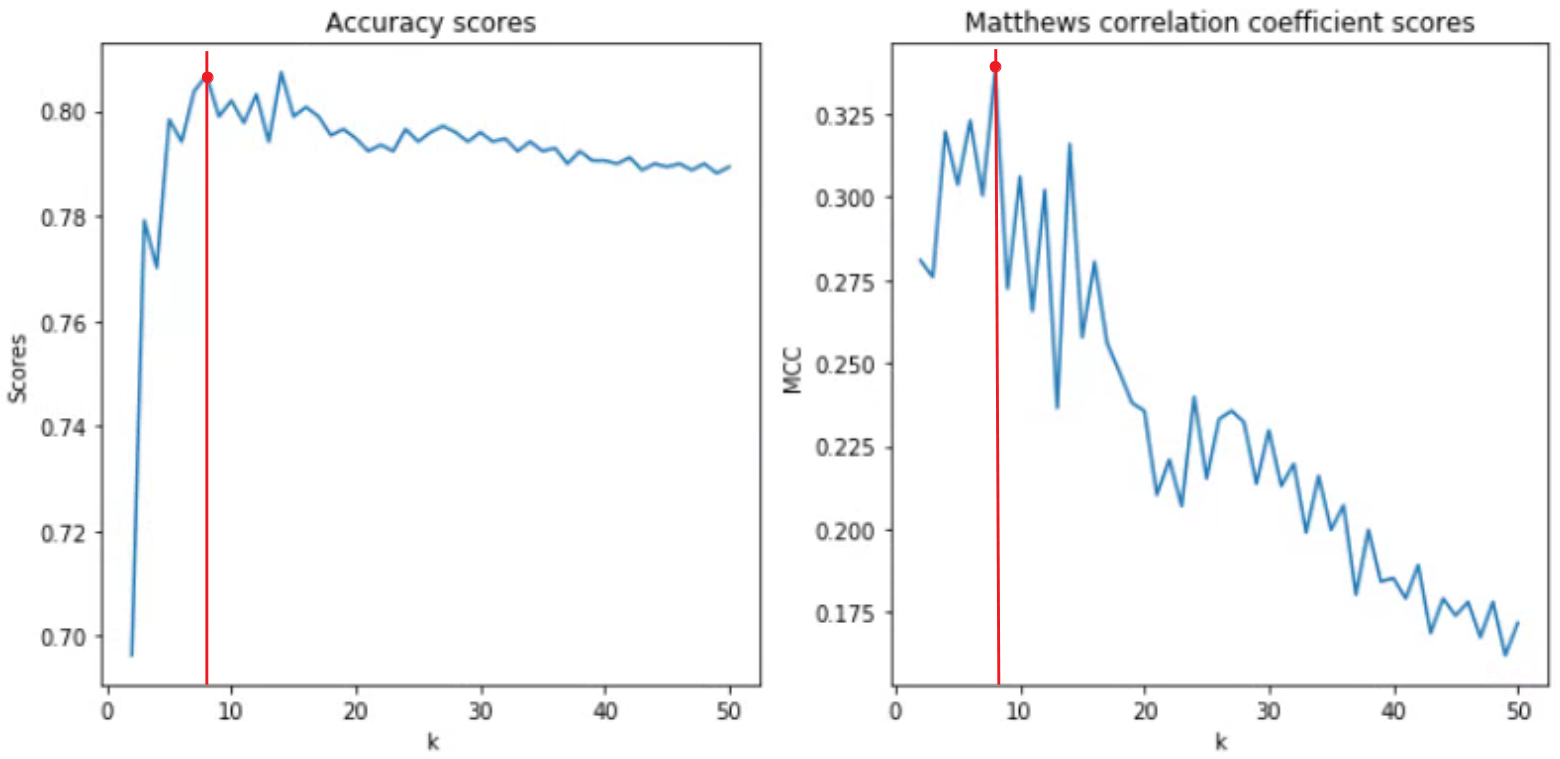
\includegraphics[width=.7\linewidth]{ThesisTemplate/Images/KNN_n_neighbors.png}
    \caption{Finding the optimum number of neighbors}
\end{figure}

\subsection{K-Modes Clustering Scenarios}
\label{ssec:cluscen}
\begin{table}[H]
\begin{footnotesize}
\begin{tabular}{llllll}
\toprule
\textbf{Scenario}   & \textbf{Features (\textit{X})}    & \textbf{Labels (\textit{y})}  & \textbf{Clusters} & \textbf{Accuracy} & \textbf{MCC}        \\
\midrule
baseline            & users + jobs                      & labels                        & -                     & 0.81              & 0.44            \\
baseline            & users                             & labels                        & -                     & 0.71              & 0.03            \\
baseline            & jobs                              & labels                        & -                     & 0.84              & 0.53            \\
\midrule
1                   & users + jobs + user clusters      & labels                        & 225                   & 0.81              & 0.41            \\ %6.7
2                   & jobs + user clusters              & labels                        & 275                   & 0.82              & 0.49            \\ %6.15
3                   & users + user clusters             & labels                        & 300                   & 0.75              & 0.08            \\ %6.8
4                   & user clusters                     & labels                        & 100                   & 0.77              & 0.05            \\ %6.13
5                   & users + jobs + job clusters       & labels                        & 225                   & 0.82              & 0.45            \\ %6.2
6                   & users + job clusters              & labels                        & 300                   & 0.77              & 0.27            \\ %6.3
7                   & jobs + job clusters               & labels                        & 250                   & 0.84              & 0.55            \\ %6.14
8                   & job clusters                      & labels                        & 150                   & 0.79              & 0.27            \\ %6.12
9                   & users                             & job clusters                  & 25                    & 0.15              & 0.11            \\ %6.4
10                  & users + jobs                      & job clusters                  & 25                    & 0.93              & 0.92*            \\ %6.6
12                  & jobs                              & user clusters                 & 25                    & 0.11              & 0.05            \\ %6.10 
13                  & users + jobs                      & user clusters                 & 25                    & 0.89              & 0.88*            \\ %6.11
\bottomrule
\tiny{*Overfitting} \\
\end{tabular}

\end{footnotesize}
\caption{\label{tab:clusc} K-Modes Clustering Scenarios \& Results}
\end{table}

\subsection{Hierarchical Clustering Scenarios}
\label{ssec:hieclu}
\begin{table}[H]
\begin{footnotesize}
\begin{tabular}{lllll}
\toprule
\textbf{Scenario}   & \textbf{Features (\textit{X})}    & \textbf{Labels (\textit{y})}  & \textbf{Accuracy} & \textbf{MCC}        \\
\midrule
baseline            & users + jobs                      & labels                        & 0.81              & 0.44            \\
baseline            & jobs                              & labels                        & 0.84              & 0.53            \\
\midrule
1                   & users + jobs + job clusters       & labels                        & 0.81              & 0.41            \\ %6.2
2                   & users + job clusters              & labels                        & 0.74              & 0.10            \\ %6.3
3                   & jobs + job clusters               & labels                        & 0.83              & 0.48            \\ %6.14
4                   & users                             & job clusters                  & 0.25              & 0.04            \\ %6.4
5                   & users + jobs                      & job clusters                  & 0.71              & 0.66            \\ %6.6
\bottomrule
\end{tabular}

\end{footnotesize}
\caption{\label{tab:hieclu} Hierarchical Clustering Scenarios \& Results}
\end{table}


\subsection{Confusion Matrices}
\label{ssec:cm}
\begin{table}[H]
\begin{footnotesize}
\begin{tabular}{llrr}
    \toprule
    \textbf{Algorithm}                  &                           &                           &                           \\
    \midrule
    Nearest Neighbors                   &                           & Positive Labels           & Negative Labels            \\
                                        & Positive Labels           & 5,482                     & 1,008                      \\
                                        & Negative Labels           & 982                       & 793                        \\
    \midrule
    K-Nearest Neighbors                 &                           & Positive Labels           & Negative Labels            \\
                                        & Positive Labels           & 1,184                     & 56                         \\
                                        & Negative Labels           & 259                       & 112                        \\
    \midrule
    RandomForest                        &                           & Positive Labels           & Negative Labels            \\
                                        & Positive Labels           & 1,203                     & 37                         \\
                                        & Negative Labels           & 256                       & 115                        \\
    \midrule
    Logistic Regression                 &                           & Positive Labels           & Negative Labels            \\
                                        & Positive Labels           & 1,155                     & 85                         \\
                                        & Negative Labels           & 241                       & 130                        \\
    \midrule
    Linear Support Vector Classification&                           & Positive Labels           & Negative Labels           \\
                                        & Positive Labels           & 1,158                     & 82                        \\
                                        & Negative Labels           & 249                       & 122                       \\
    \midrule
    Neural Network                      &                           & Positive Labels           & Negative Labels           \\
                                        & Positive Labels           & 1,129                     & 111                       \\
                                        & Negative Labels           & 190                       & 181                       \\
    \midrule
    \textit{Legend}                     &                           & Positive Labels           & Negative Labels            \\
                                        & Positive Labels           & \textit{True positives}   & \textit{False negatives}   \\
                                        & Negative Labels           & \textit{False positives}  & \textit{True Negatives}    \\
    \bottomrule
\end{tabular}
\end{footnotesize}
\caption{\label{tab:cm} Confusion Matrices}
\end{table}